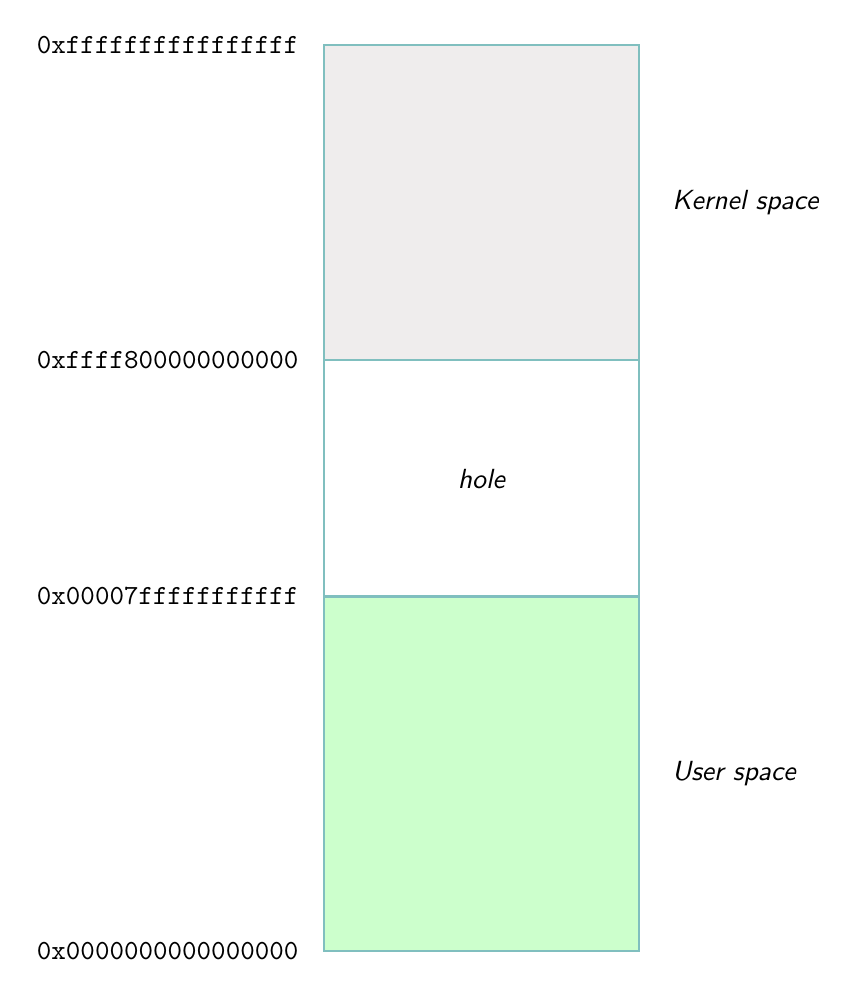
\begin{tikzpicture}[
    % Estilos de las cajas (colores suaves mezclados)
    userbox/.style={thick, draw=teal!50, fill=green!20},
    holebox/.style={thick, draw=teal!50, fill=white},
    kernelbox/.style={thick, draw=teal!50, fill=pink!15!gray!15},
    % Estilos para los textos
    addr/.style={font=\ttfamily, text=black, anchor=east},
    labeltext/.style={font=\sffamily\itshape, text=black, anchor=west}
]

% --- USER SPACE ---
\draw[userbox] (0, 0) rectangle (4, 4.5);
\node[labeltext] (user) at (4.3, 2.25) {User space};
\node[addr] (addr1) at (-0.2, 0) {0x0000000000000000};
\node[addr] (addr2) at (-0.2, 4.5) {0x00007fffffffffff};

% --- HOLE ---
\draw[holebox] (0, 4.5) rectangle (4, 7.5);
\node[font=\sffamily\itshape, text=black] (hole) at (2, 6) {hole};

% --- KERNEL SPACE ---
\draw[kernelbox] (0, 7.5) rectangle (4, 11.5);
\node[labeltext] (kernel) at (4.3, 9.5) {Kernel space};
\node[addr] (addr3) at (-0.2, 7.5) {0xffff800000000000};
\node[addr] (addr4) at (-0.2, 11.5) {0xffffffffffffffff};

\end{tikzpicture}